% THIS IS SIGPROC-SP.TEX - VERSION 3.1
% WORKS WITH V3.2SP OF ACM_PROC_ARTICLE-SP.CLS
% APRIL 2009
%
% It is an example file showing how to use the 'acm_proc_article-sp.cls' V3.2SP
% LaTeX2e document class file for Conference Proceedings submissions.
% ----------------------------------------------------------------------------------------------------------------
% This .tex file (and associated .cls V3.2SP) *DOES NOT* produce:
%       1) The Permission Statement
%       2) The Conference (location) Info information
%       3) The Copyright Line with ACM data
%       4) Page numbering
% ---------------------------------------------------------------------------------------------------------------

\documentclass{acm_proc_article-sp}
\usepackage{lmodern} % font problem fix

\usepackage{subcaption}
\usepackage{graphicx}
\usepackage{float,dblfloatfix,fixltx2e}
\usepackage[format=plain,font=small,labelfont=bf]{caption}
\usepackage[utf8]{inputenc}
% noitemsep option for enumerate and itemize
\usepackage{enumitem}
\usepackage[backend=biber]{biblatex}

% typesetting algorithms
\usepackage{algorithmicx}
\usepackage[noend]{algpseudocode}
\usepackage[section]{algorithm}

% grammar?
\usepackage{syntax, etoolbox}
\AtBeginEnvironment{grammar}{\small}
\setlength{\grammarparsep}{8pt plus 1pt minus 1pt}
\setlength{\grammarindent}{12em}

\addbibresource{sources.bib}

% real code
\usepackage{listings,color,xcolor}
\usepackage{lstlang0} % go
\definecolor{dkgreen}{rgb}{0,0.6,0}
\usepackage{MnSymbol}
\usepackage[hidelinks]{hyperref}
\lstset{
	prebreak=\raisebox{0ex}[0ex][0ex]{\ensuremath{\rhookswarrow}},
	postbreak=\raisebox{0ex}[0ex][0ex]{\ensuremath{\rcurvearrowse\space}},
	breaklines=true,
	numbers=left,
	numberstyle=\scriptsize,
	breakatwhitespace=true,
	frame=single,
%	frameround=tttt,
	tabsize=4,
	showstringspaces=false,
	aboveskip=1.8em,
	belowskip=0em,
	captionpos=b,
	xleftmargin=0.4em,
	xrightmargin=0em,
	keywordstyle=\bfseries\color{dkgreen},
	commentstyle=\itshape\color{purple},
	identifierstyle=\color{black},
	stringstyle=\color{blue},
	basicstyle=\small\ttfamily
}

\lstdefinelanguage{Paratype}{
	morekeywords={func,inherits,implements,throws,type,typeclass,constrain,to},
}
\lstdefinelanguage{Gopp}{
	%keywords={=>,=,*,+},
	comment=[l]{\#\#},
	morestring=[b]{'},
%	moredelim=*[s]{(}{)},
%	moredelim=*[s]{<}{>},
}


\begin{document}

\title{Paratype --- A Parallel Type Completion System}


% You need the command \numberofauthors to handle the 'placement
% and alignment' of the authors beneath the title.
\numberofauthors{3}
\author{
\alignauthor
Tyler Cecil\\
       \affaddr{New Mexico Tech}\\
       \affaddr{801 Leroy Place}\\
       \affaddr{Socorro, NM 87801 USA}\\
       \email{tcecil@nmt.edu}
\alignauthor
Ben Turrubiates\\
       \affaddr{New Mexico Tech}\\
       \affaddr{801 Leroy Place}\\
       \affaddr{Socorro, NM 87801 USA}\\
       \email{bturrubi@nmt.edu}
\alignauthor
Christopher Koch\\
       \affaddr{New Mexico Tech}\\
       \affaddr{801 Leroy Place}\\
       \affaddr{Socorro, NM 87801 USA}\\
       \email{ckoch@cs.nmt.edu}
}
\date{\today}

\maketitle
\begin{abstract}
  In the following report we introduce \emph{Paratype}, an actor model of
  type completion. Type analysis of modern languages such as
  Haskell, Agda, and Coq can be an intense stage in compilation. % CITE
  With the use
  of an actor model, we may cut down compilation time as well as open up
  doors for new models of type evaluation. Working on a grammar with bounded
  parametric polymorphism, Paratype communicates types across a large call
  graph to resolve type errors, append errors, and evaluate types in parallel.
  To minimize message overhead, we have used a shared memory message
  passing system. We believe our actor approach significantly
  speeds up the compilation process and it may apply to some other interesting
  problems.
\end{abstract}

\category{F.3.3}{Studies of Program Constructs}{Type structure}
\category{D.3.3}{Programming Languages}{Language Constructs and Features}
\category{D.3.4}{Programming Languages}{Processors}

% some out of 16 general terms!
\terms{Design, Languages, Performance}

\keywords{type theory, language theory, type completion, type checking, type
inference, code analysis, parallel, actor model}

\section{Introduction}

% problem and why important
% compilers: e.g. just-in-time comp

``Compile one time, run many times: that means compilers do not need to be
fast, right?'' Luckily, no software engineer thinks this way. In fact,
compilation speed is a concern of many budding languages. Aside from lexing,
typically the slowest part of compilation, modern
languages spend an embarrassing amount of time resolving
types. % CITE (tyler)
Principally, this is due to the adoption of the
\emph{System F} formalization in modern strongly typed languages. Moreover,
many languages have type inference or even type bounds, further complicating
the process. Unfortunately, type evaluation serves as the foundation for
automated theorem provers and other logic analysis systems. Even within the
compilation domain, interpreted languages and JIT languages need type
resolution much faster than is currently being provided. Type evaluation needs
to be expedited.

To achieve this, we have developed \emph{Paratype}: an actor model of
type evaluation. As will be apparent shortly, most type evaluation procedures
can be described as a conversation between functions. Each function
communicates information about its type to ``neighboring'' functions. As the
chatter subsides, we are left with all functions knowing their types or a
function knowing that it cannot compile. Most systems involve walking through
the tree of this conversation. Using a shared memory message passing system,
\emph{Paratype} allows functions to be actors and lets the conversation
happen.

At the moment, we are only using a toy grammar that is defined in the
proposal. Our grammer includes types of normal variables, and error types in
order to cover most use cases in modern type systems. Perhaps one day
\emph{Paratype} can be integrated into a project such as the Haskell
compiler \texttt{ghc}.

\section{Problem Definition}
\label{sec:problem}
% grammar, input/output, type completion, lambda calculus (System F)

Formally, our problem will be to take an input file of a specified grammar and
generate an output of either failure due to undecidability or the same file
with multiple implementations of each function for each set of explicit types
instead of type variables. In the process of doing this, we will also be
performing type checking. The goal is to find an explicit type for
each function call without type conflicts.

We define a few terms to use throughout the proposal:
\begin{description}
	\item[Type] A set of values. Types may implement type classes.
	\item[Type class] A set of types. Type classes may inherit other type classes.
	\item[Context] The set of explicit types and metainformation associated
		with a function call: caller, parameter types, return type.
	\item[Resolution] Resolving a context means giving it explicit types.
	\item[Parent (function)] Caller of a function.
	\item[Child (function)] A function that is called by its parent function.
	\item[Type variable] A variable that ranges over types. A type variable may
		be constrained to zero or more type classes.
	\item[Parametric polymorphism] A way to allow a language to express the
		handling of functions and types homogeneously independent of their type
		through the use of generic functions, also known as generic
		programming.
	\item[Bounded parametric polymorphism] A method of providing extra
		information about a generic data type. In Haskell, this is achieved by
		creating a type class which types may implement.
\end{description}

Listing~\ref{lst:informalg} shows an informal example of our grammar. It is a
grammar for a simple functional language that provides bounded parametric
polymorphism through type classes. This allows expressing functions in terms of
generic types while still maintaining the same behavior. This use of type
variables introduces the need for partial contexts.

\begin{lstlisting}[caption=Grammar displayed informally,language=Paratype,label=lst:informalg]
typeclass Arithmetic
typeclass Num inherits Arithmetic

type int implements Num
type float implements Num

func foo(int, T, R) float throws errorType
    = bar(baz(T), R, int)
\end{lstlisting}

An example of a partial context is shown in Listing~\ref{lst:cbyparent}. The
function \lstinline!bar! is declared as accepting and returning a \lstinline!T!
type.  This introduces a partial context due to \lstinline!T! being a type
variable. The parameter type for \lstinline!bar! is provided by its parent
function \lstinline!foo!. This also completes the return type of
\lstinline!bar!.

\begin{lstlisting}[caption=Explicit context provided by parent,language=Paratype,label=lst:cbyparent]
type int
func foo(int, int) int
    = bar(int)

func bar(T) T
    = T
\end{lstlisting}

Types for partial contexts can be provided by both the parent and the child.
Consider the example shown in Listing~\ref{lst:cbychild}. Function
\lstinline!foo!  is defined as returning an \lstinline!R! type. The function
definition contains the result of calling \lstinline!bar! as the return value.
\lstinline!bar! is defined as having an \lstinline!int! return type. Since
\lstinline!foo! returns the value of calling \lstinline!bar! it also has a
return type of \lstinline!int!.

\begin{lstlisting}[caption=Explicit context provided by child,language=Paratype,label=lst:cbychild]
type float
type int
func foo(T, S) R
    = bar(T, S)

func bar(float, float ) int
    = int
\end{lstlisting}

In the previous examples all partial contexts have been resolved by either the
parent or the child. There are situations where they can mutually provide
contexts for each other. One example of this is shown in
Listing~\ref{lst:cbyboth}. In this example \lstinline!foo! is providing
the type of the second parameter for function \lstinline!barbar!.
\lstinline!barbar!  also provides the type of the first parameter for function
\lstinline!foo!. Notice that function \lstinline!barbar! is defined as
returning a type variable \lstinline!R!. Since \lstinline!foo! returns an
\lstinline!int! type and its return value is a call to \lstinline!barbar!; this
resolves the return type for \lstinline!barbar!. The evaluation of these
partial contexts is a non-trivial task.

\begin{lstlisting}[caption=Explicit context provided by child and parent,language=Paratype,label=lst:cbyboth]
type int
func foo(T, int) int
    = barbar(T, int)

func barbar(int, T) R
    = R
\end{lstlisting}

Another problem that type variables introduce is the need to maintain partial
contexts. Multiple fully evaluated contexts may exist in the end and may not be
the result of type errors. An example of this is shown in
Listing~\ref{lst:partial}. The \lstinline!bar! function accepts a type variable
\lstinline!b! as an input parameter. The function \lstinline!foo! provides a
context for \lstinline!bar! in which \lstinline!b! is of type \lstinline!int!.
At this point \lstinline!bar! now has a fully evaluated context, but
\lstinline!baz! can also complete the partial context with \lstinline!b!
resolving to type \lstinline!float!.  In this situation these are both valid
and should not be considered a type error.

\begin{lstlisting}[caption=Need to maintain partial contexts,language=Paratype,label=lst:partial]
type char
type int
type float
func foo(int) T
    = bar(int)

func bar(T) char
    = char

func baz(float) T
    = bar(float)
\end{lstlisting}

Although contexts can be provided by both the parent and the child, there are
situations where there is not enough information to resolve a context. Consider
Listing~\ref{lst:unhalting}: \lstinline!bar! accepts a type variable as a
parameter. The context provided by its calling function \lstinline!foo!
resolves the parameter as being the local variable \lstinline!b!. This is
problematic due to \lstinline!b! also being a type variable. In this example
there is not enough information to resolve a full context for either
\lstinline!bar! or \lstinline!foo!.

\begin{lstlisting}[caption=Unhalting context resolution,language=Paratype,label=lst:unhalting]
type int
func foo(T) int
    = bar(T)

func bar(T) int
    = int
\end{lstlisting}

Introducing errors into the grammar adds more complexity. In the example shown in Listing~\ref{lst:errors},
all parent functions of \lstinline!bar! need to have \lstinline!weirdError! in
their fully resolved contexts.

\begin{lstlisting}[caption=Errors,language=Paratype,label=lst:errors]
func foobar(T b) T
    = foo(b)

func foo(int b) int
    = bar(b)

func bar(T a) T throws weirdError
    = T
\end{lstlisting}

% ADD EXAMPLE OF NESTED FUNCTIONS
\section{Methods}

% Google Go and why

Due to the actor model, the problem lends itself nicely to a distributed memory
approach; however, it is usually commodity hardware that is used for
compilation. Therefore, used Google Go due to its concept of
\texttt{goroutines}. A \texttt{goroutine} is a lightweight thread that is
managed by the Go runtime.

\begin{lstlisting}[caption=Small \texttt{goroutine} example with
\texttt{channels},language=Go,label=lst:goroutine]
func node(name string, c chan string) {
	fmt.Println("I'm node ", name)
	/* send message to c
	 * (blocks until receiver is ready)
	 */
	c <- strings.Join(name, " has a message for you.")
}

func main() {
	// unbuffered channel
	c := make(chan string)
	go node("abc", c)
	// receive message from c (blocks)
	a := <-c
	fmt.Println(a)
}
\end{lstlisting}

It is possible to pass references through shared memory, called
\texttt{channels}, with \texttt{goroutines}: like message passing in shared
memory. This can be seen in Listing~\ref{lst:goroutine}. Of course, unlike in
the example, the channel may also be buffered and would thus only block sending
when the buffer is full and receiving when the buffer is empty. This is one of
the reasons that we chose Google Go: it allows us to use message passing
with a high degree of flexibility without the overhead of actually sending the message.

% TODO: talk about interesting go features like WaitGroups etc
% TODO: was Go a good idea?

The \texttt{goroutines} fit the actor model of type resolution nicely since the
threads are lightweight and communication is easy to arrange. We found
ourselves taking advantage of the fact that messages sent and received through
\texttt{channels} are actually references to shared memory. This way, a
specific context will update everywhere that it is referenced and we must only
notify other actors that something changed instead of sending the context
again. This reduces communication overhead while still functioning as a message
passing system.

Go also provides concurrency features that are useful for managing state. One
of these concurrency primitives is the \texttt{WaitGroup}. A \texttt{WaitGroup}
essentially consists of a semaphore; there is a method to increment it and a
method to decrement it. The peculiar addition is a wait method: the wait method
will block until the semaphore in the \texttt{WaitGroup} is decremented to
zero.

Paratype makes use of \texttt{WaitGroup}s in several places. For example, for
function composition, a function's composed context is evaluated from the
innermost composed function(s) to the outermost composed function sequentially:
the function actor resolving its function composition must wait for the
innermost functions to resolve context before moving on to the next ``level''
of the composition. It does so by sending a pointer to a \texttt{WaitGroup}
with its message to the children of the composition. These children will send
to their children and this repeats until the message has trickled all the way
down the tree to the leafs (functions with no children). Each of these leafs
decrement the \texttt{WaitGroup}. When every leaf has done that, the
composed function that sent the message will be released from its wait call on
the \texttt{WaitGroup} since the wait method will unblock when the semaphore is
zero. The composing function then knows that it may move on to the next level
of function composition.

% TODO : Discuss Clojure as a viable alternative and analyze whether the
% decision to use Go was the correct one.

Although Go provides nice concurrency features, we sometimes found ourselves
fighting with the type system and verbosity of the language. Another
consideration for the implementation could have been \texttt{Clojure}. Clojure
is a lisp variant that runs on the Java Virtual Machine. There is a library for
Clojure, \texttt{core.async}, which implements some concurrency features that
are  modeled after Google Go's concurrency system. This brings the same shared
memory channels with the advantages of the concise and dynamic nature of
Clojure. Clojure is also built for concurrency and boasts immutable data types
to provide safety in parallelized code. One of the issues with this is that
Paratype is a very state-driven application. This could lead to performance
faults when using a language that is not built for modeling mutable state.


\section{Parallelization}

The algorithm that is the heart of Paratype works in essence as following.
Steps preceded by ``--'' are performed in parallel.
\begin{description}[noitemsep]
	\item[Parsing] Parse input file according to Paratype grammar.
	\item[Setup] For each function, collect context information by finding type
		variables and function calls as well as the relation of type variables
		from function declaration to function calls
	\item[Goroutines] For each function, spawn a goroutine (function actor) and
		do:
	\item[-- Initial send] Each function actor will send context information
		about its function to all its children (callees). See details in
		Subsections~\ref{subsec:typeresolution} and~\ref{subsec:funccomp}.
	\item[-- Type resolution] Each function actor listens for messages,
		performs merging, and sends the message to its children. See details
		in Subsection~\ref{subsec:typeresolution}.
	\item[-- Halting type resolution] Wait for each function actor to finish
		resolving types. See details in Subsections~\ref{subsec:halting}
		and~\ref{subsec:errorhalting}.
	\item[-- Implementation collection] Close all channels of communication,
		which acts as an implicit barrier for all function actors to walk up
		their call tree to collect sets of explicit types for themselves.
	\item[-- Halting collection] Wait for all function actors to finish
		implementation collection.
	\item[Printing] Printing the implementations.
\end{description}

\subsection{Type Resolution}
\label{subsec:typeresolution}

This is what each function actor $f$ does during its runtime:
\begin{enumerate}[noitemsep]
	\item Receive path-context object $(P, C_h)$ from parent $g$, where the
		path is the path that the context has traveled so far and the context
		$C_h$ is the context of some function $h$.
	\item Merge type information from $C_f$ into $C_h$.
	\item Add $f$ to path $P$ and send $(P, C_h)$ to all children of $f$.
\end{enumerate}

Merging type information from $C_f$ into $C_h$ is a tricky task. There are two
cases:
\begin{enumerate}
	\item If $h$ is a direct parent of $f$, the function call from $h$ to $f$
		can be matched to $f$'s declaration.

		$f$ will override the type
		variables of that function call with the ones generated through its
		declaration and remember which ones it replaced by storing them in a
		map (called the type variable map).

		It will then override the type variables of $h$ that were used in the
		call to $f$ as well. $f$ knows which ones to replace: if a type
		variable in the declaration of $h$ is a key in its type variable map,
		it will replace it with the corresponding value.
	\item If $h$ is not a direct parent of $f$, we will simply use the type
		variable map created through direct parents of $f$ as detailed
		previously to replace any type variables in $h$.
\end{enumerate}

Ultimately, this allows type variables from the leaf nodes of the call graph to
``trickle up'' through the nodes until finally, the roots of the call graph and
every node in between is related to a leaf.

\subsection{Implementation Collection}

In the implementation collection phase, each function walks up its call tree to
find explicit sets of implementations for itself. If it reaches a function
without parents that does not have an explicit implementation, it will throw a
type error denoting this. Due to function composition, the implementation
collection phase is actually a bit more complicated than this: Each function
actor will also look at the type variable maps it encounters to find equivalent
type variables to look for when trying to find implementations of itself.

\section{Parallel Design}
	This section details some of the more difficult parallel design decisions
	made in addition to the algorithmic design.

	\subsection{Making Halting Deterministic}
		\label{subsec:halting}

		An issue when performing the type completion and analysis in parallel
		is knowing when all of the operations are completed and halting can
		commence.

		Halting in the initial implementation of Paratype was simple but wrong:
		each of the function actors spawned had a reference to a
		\texttt{WaitGroup} which they incremented when they did work and
		decremented when they did not. The main function would then wait for
		all actors to become inactive, at which point it would check that all
		channels were empty.  Obviously, this is a race condition: between the
		activity check and the checking of the channels, a function actor may
		have read the last message from the channels and thus become active
		while the channels are empty.

		In the current version of Paratype, there are two main steps separated
		by an implicit barrier: the type resolution step and the implementation
		collection step. Halting for the implementation collection step is
		trivial, but halting in the type resoltion step is more complicated.

		In that step, halting takes advantage of the fact
		that communication only happens from callers to callees. Function
		actors which are not called from anywhere know that after they gather
		their context information and send it to all their children, they will
		never receive any messages since only their callees may send them
		messages. Thus, they can mark themselves as done. They communicate this
		to their children in their last transmission.

		Any function actor which has parents will wait for all their parents to
		be done. Once they process all their messages, they then know that they
		cannot receive any more messages and can mark themselves as done. They
		will communicate this to their children as well.

		Every function actor has a channel back to the main thread for sending
		type errors once they arise. This channel is also used to signal the
		main thread that a function actor is done: instead of an error, a
		function actor that is done will send \lstinline!nil! (similar to a
		\lstinline!NULL! pointer) back to the main thread. The main thread will
		keep track of how many function actors are active and once every
		function actor is inactive, we can enter the implementation collection
		step.

% 		\begin{lstlisting}[caption=Communication Struct, language=Paratype, label=lst:commstruct]
% type Communication struct {
% 	Path		string
% 	Context		*Function
% 	Depth		int
% 	LastComm	bool
% 	Wait		*sync.WaitGroup
% }
% 		\end{lstlisting}
	\subsection{Halting On Type Error Detection}
		\label{subsec:errorhalting}

		Even though the previously described implementation for halting may
		work on valid input, it fails for input that generates a type error.
		One of the advantages of performing the type checking process in
		parallel is that type errors can be detected earlier, but once a type
		error is detected, all threads must all exit gracefully.

		When a function actor encounters a type error during its type relation
		compilation step, it will signal this to the main thread using the
		previously described error channel and stop computation. The problem
		then is that the main thread needs a way to stop all other function
		actors: Google Go does not provide any facilities for stopping a
		running goroutine or for checking whether a communication channel is
		closed. With that in mind, simply closing all channels of communication
		is out of the question.

		To approach the problem, every function actor was provided with a
		reference to a global \texttt{WaitGroup} and a boolean representing
		whether execution should stop. The main thread will set the boolean to
		true when every function actor should stop executing. Simply checking
		the boolean before trying to send to a channel is a race condition,
		though, which is where the \texttt{WaitGroup} comes in: when the main
		thread learns of a type error, it will increment the \texttt{WaitGroup}
		and before a function actor tries to send a channel, it calls wait on
		the \texttt{WaitGroup}. After incrementing the \texttt{WaitGroup}, the
		main thread will set all the booleans to true and then release the
		\texttt{WaitGroup}. After this, we know that no thread will try to send
		to any channel and the main thread may close all function actor
		channels as well as error channels.

	\subsection{Function Composition}
		\label{subsec:funccomp}

		One of the issues induced by parallelization is the handling of
		function composition. Consider the code snippet shown in
		Listing~\ref{lst:composition}.

		\begin{lstlisting}[caption=Small Example of function composition,
		language=Paratype, label=lst:composition]
type int
type float
type boat
func f(A) boat
	= g(m(A), h(A), int)
func g(B, C, B) D
	= D
func m(int) A
	= A
func h(A) float
	= float
		\end{lstlisting}

		In the initial implementation of Paratype, a function with no parents
		(an aristocratic function) did not need to have a thread spawned for
		itself, since the ``initial send'' step of the algorithm would send its
		first (and thus, last) message before the goroutines were created.

		However, function composition made this optimization obsolete: The
		children would all evaluate their own contexts and replace type
		variables in their parents while other children were trying to do the
		same: even though there was a read-write mutex in place, children now
		did not know the relation of their type variables to those in the
		parents anymore if another child overwrote it and could thus not
		resolve their types. This would cause the evaluation to be unresolvable
		due to inability to correctly find relations between type variables.

		This was solved using a technique we refer to as ``in-out evaluation:''
		any function actor that contains function composition will send to the
		innermost children of the composition first and then wait for those
		children to finish resolving types. Once that happens, it then sends
		to the next level of the composition (second-to-inner) and the process
		repeats until finally the outermost function is resolved.

		The way the children signal that they are done resolving types is
		through a wait group (like a semaphore) that they decrement. The parent
		will be blocking on a wait call that unblocks once the semaphore is
		equal to zero, then knowing that the respective level of composition is
		done resolving and that it may go up one level.


\section{Verification}
	All of our testing was performed with curated examples that were picked to
	intentionally pose a problem and ensure that each of the subsystems were
	working correctly. When the completion is performed the output is written
	to a file. These files can then be checked for correctness. Go provides a
	useful testing package that allows for executing all tests or selected
	tests.  It launches the threads and gives details about execution and gives
	the state of the goroutines during an error. This is incredibly useful and
	was used often to test the hand-made examples. It was not uncommon to also
	repeatedly run these tests to ensure they were deterministic in halting and
	not causing exceptional situations.

\section{Analysis and Model}
%  variables: number of functions, function calls, contexts, partial contexts,
%  undecidability, number of physical cores available, number of types and type
%  classes, etc

For analysis, some of the previously mentioned examples were timed for numbers
of processors as powers of two up to 32 processors, whereas each timing was
repeated 30 times. The tests were run on \texttt{login.cs.nmt.edu}, a machine
with two CPU cores. Even though there was huge variation for a
fixed problem size and a fixed number of processors, speedup was obtained by
using the average of the time taken for one processor as the sequential time.

Even though we expected a good amount of speedup from our model, initial
results are not hopeful: For very small examples, speedup is limited to two or
four processors and sublinear, as can be seen in Figures~\ref{fig:c1s}
and~\ref{fig:c3s}.

In fact, for anything above two or four processors, our model would slow down.
For 32 processors, it took almost 10 times as much time to resolve types than
it did for one processor. To explain this behavior we can look at two
main factors: our input files and the Go Scheduler.

\subsection{Input File Generation}

In the case of our input files, most of our performance can be
attributed to a distinct lack of size and diversity of our
problems. To properly achieve a quality analysis we would need to be
able to readily vary parameters such as number of functions, number of 
function compositions, number of errors, number of type variables, number of
type classes, etc. Unfortunately, we were unable to build problems
of large enough sizes to take advantage of all of our threads. This
does not explain our apparent ``slow down''; to tackle that we need to
understand the Go Scheduler.

\begin{figure}[ht]
	\centering
	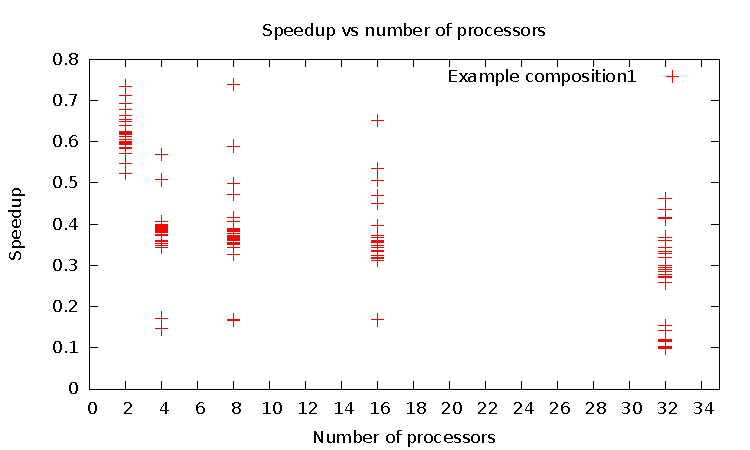
\includegraphics[scale=0.6]{../../data/composition1s.pdf}
	\caption{Speedup vs number of processors, example composition1 (four
	functions)}
	\label{fig:c1s}
\end{figure}

\begin{figure}[ht]
	\centering
	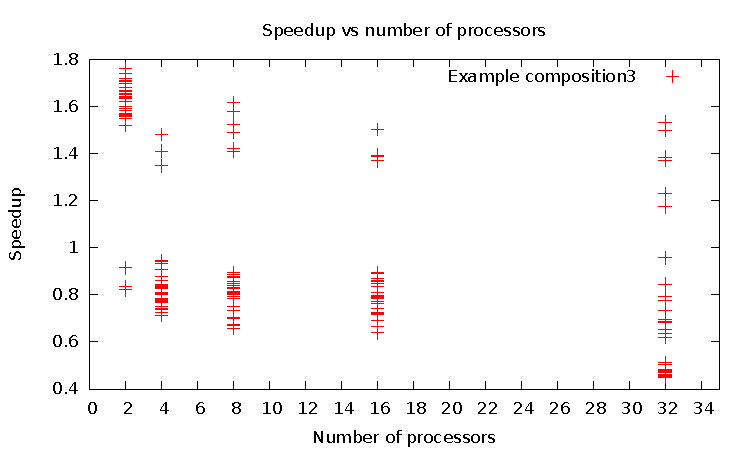
\includegraphics[scale=0.6]{../../data/composition3s.pdf}
	\caption{Speedup vs number of processors, example composition3 (84
	functions)}
	\label{fig:c3s}
\end{figure}

\begin{figure}[ht]
	\centering
	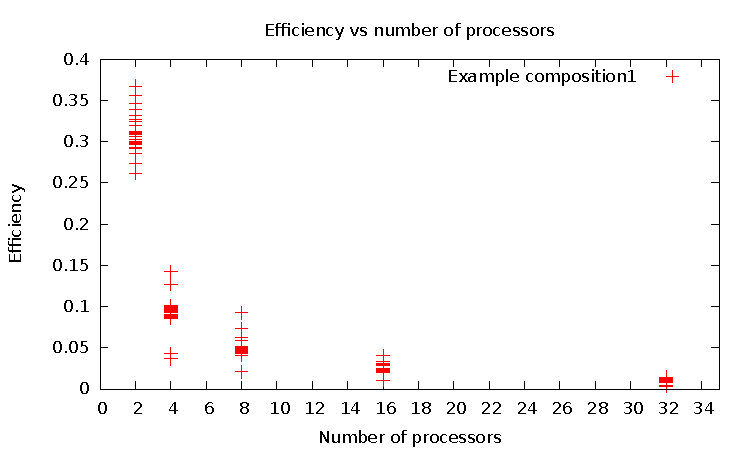
\includegraphics[scale=0.6]{../../data/composition1e.pdf}
	\caption{Efficiency vs number of processors, example composition1 (four
	functions)}
	\label{fig:c1e}
\end{figure}

\begin{figure}[ht]
	\centering
	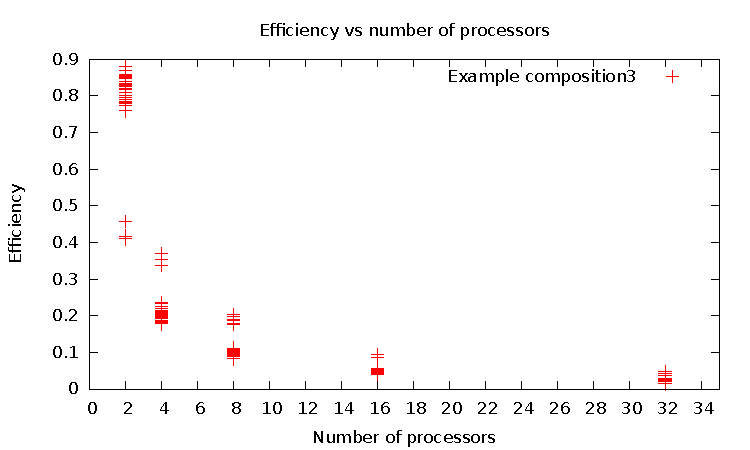
\includegraphics[scale=0.6]{../../data/composition3e.pdf}
	\caption{Efficiency vs number of processors, example composition3 (84
	functions)}
	\label{fig:c3e}
\end{figure}
\subsection{The Go Scheduler}

The Go Scheduler was designed by Dmitry Vyukov. In a normal shared
memory system such as \emph{OpenMP}, a scheduler would not be
necessary. The operating system will simply allocate threads and
schedule them as they would any other process. However, pthreads require a huge
amount of overhead since they are almost full OS processes.

In Go it is not uncommon to have thousands of go routines running and that
overhead can build up. Because of this and the fact that go has insight into
the behavior of the code and can more properly schedule tasks, Go compiles its
own scheduler into the binary\cite{go-sched}.

A suspect to our loss of speed would be work stealing. Go uses $M:N$
scheduling, meaning $M$ threads will be mapped to $N$ Pthreads \cite{go-sched}.
With a large number of threads, there will only be so many tasks allocated to
each thread. Therefore, when a thread runs out of tasks, they will attempt
to invoke work stealing. At large values of \texttt{GOMAXPROCS}, work
stealing will happen constantly, dragging down our execution speeds.

Due to time constraints, not a lot of data was collected about performance. One
can see in the figures that the example composition3 had better speedup for two
and four processors than composition1; this is likely due to the fact that it
had more functions. We would expect that once the systems become more
complicated and connected, the speedup would increase for a higher number of
processors; it is likely that the overhead of 32 \texttt{goroutines} and the Go
scheduler are not beneficial for anything above four processors.

Since speedup was not very good; of course efficiency was even worse. See
Figures~\ref{fig:c1e} and~\ref{fig:c3e}.


% variables: number of functions, function calls, contexts, partial contexts,
% classes, etc
%
% gopp parser hangs in some cases (not our focus, so we don't care)
%
%just some notes to use for empirical analysis later
%
% Complexity of f.Update(g) algorithm if g is parent of f: \[ U(f, g) =
% \sum_{\textrm{v in args of g and w replaces v}} V(v, w)) \leq O(|\textrm{num
% args of g}| \times |\textrm{num typeclasses}|) \]
%
% UpdateTypevar (v and w merge to w): \[ V(v, w) = O(|\textrm{num of
% typeclasses on w}|) \]
%
% Complexity of f.Update(g) if g is parent of f: \[ \leq O(|\textrm{num atlas
% entries of g}| \times |\textrm{num typeclasses}|) \]
%
% All of these multiplied by hashmap access time at worst $O(\textrm{size of
% map})$ each
%
% how often is f.Update(g) called?
%
% -> context path object travels down every path!
%
% -> number of paths times number of nodes in each path
%
%  gopp parser hangs in some cases (not our focus, so we don't care)

% just some notes to use for empirical analysis later

%  Complexity of f.Update(g) algorithm if g is parent of f: \[ U(f, g) =
%  \sum_{\textrm{v in args of g and w replaces v}} V(v, w)) \leq O(|\textrm{num
%  args of g}| \times |\textrm{num typeclasses}|) \]

%  UpdateTypevar (v and w merge to w): \[ V(v, w) = O(|\textrm{num of
%  typeclasses on w}|) \]

%  Complexity of f.Update(g) if g is parent of f: \[ \leq O(|\textrm{num atlas
%  entries of g}| \times |\textrm{num typeclasses}|) \]

%  All of these multiplied by hashmap access time at worst $O(\textrm{size of
%  map})$ each

%  how often is f.Update(g) called?

%  -> context path object travels down every path!

%  -> number of paths times number of nodes in each path

\section{Known Bugs}

Currently, there are four known bugs worth mentioning that are resolvable but
would be time-consuming to fix and would not require any parallel design:
\begin{itemize}
	\item Incorrect representation of function composition when printing:
		Because after parsing, only the ``level'' of composition of a function
		and its type-variable relation is kept, but not its place in the
		composition, some of the printed output is incorrect.
	\item Small bug in the implementation collection phase where a function
		actor does not actually look through all the type variable maps it
		finds to find relations to its own type variables. In most cases, this
		is insignificant, but in some function composition cases it will not
		resolve when types are resolvable. The type variable relations are
		there and have been found, they are just not connected back correctly
		to the original function in some cases.
	\item In many cases, the parser will not catch incorrectly formatted files
		or missing declarations. We currently assume that every input file is
		correctly formatted except for type errors.
	\item Sometimes, implementations are printed more than one time.
\end{itemize}

None of these bugs would require parallel design and therefore, their
resolution has not been a priority. In all cases, they require a
simple fix of representation that would be time-consuming.



\pagebreak
\section{Conclusion}

\emph{Paratype}, as is, serves as a proof of concept of a novel approach to
type analysis. It achieved its goal of being able to resolve simple merges and
function compositions, explored the design of an actor-based type system, and
helped define many of the problems that would be faced in a full type analysis
system. That being said, it still needs work to tackle all problems of a type
analysis system, most notably there is the lack of cycle detection in call
graphs. In many cases, some preliminary algorithms have been detailed to tackle
these edge cases and missing features, though they have yet to be implemented.
Finally, time needs to be taken to further optimize the existing code base;
known inefficient uses of memory and processing are current in the
\emph{Paratype} code base.

Without the means to generate complicated, feature-rich source files, a quality
analysis of the software performance can not be performed. As is, it appears
parallel overhead takes over the advantages of the software, but this was
tested only with simple examples. The algorithms that were designed in this
project were elaborate, novel, and exciting. It is our hope to continue with
\emph{Paratype} and see it to its end.

\appendix

\section{Github}

Our project can be found on Github at
\begin{center}
	\vspace{-5mm}
	\url{https://github.com/izzycecil/Paratype}
\end{center}

\section{Team Members and Their Contributions}
	\begin{description}
		\item[Ben] Ben worked on halting and function composition as well as
			parsing.
		\item[Chris] Chris worked on getting function composition working and
			the merging algorithm.
		\item[Tyler] Tyler worked on setting up communications between the
			function actors as well as initial halting.
	\end{description}

\section{Things Learnt From This Project}

	We learnt some interesting things about a new programming language and
	quite a bit of parallel debugging from this project. We took advantage of
	some new design patterns in parallel programming that are inherently
	included with Google Go, such as communication channels' closure acting as
	an implicit barrier.

	We have also learnt that relying on software libraries for certain things
	(in our case parsing) is not always as useful as it might seem. Getting the
	gopp grammar parser to work correctly took a lot more time than it should
	have and set us back by quite a bit.
\printbibliography

\balancecolumns
\end{document}
